\documentclass[9pt,twocolumn,twoside]{../../styles/osajnl}
\usepackage{fancyvrb}
\journal{i524} 

\title{Automated Sharded MongoDB Deployment and Benchmarking for Big Data Analysis}

\author[1,*]{Mark McCombe}

\affil[1]{School of Informatics and Computing, Bloomington, IN 47408, U.S.A.}
\affil[*]{Corresponding authors: laszewski@gmail.com}

\dates{S17-IO-3012, \today}

\ociscodes{MongoDB, Cloud Computing, Ansible, Python, Cloudmesh Client, Openstack, I524}

% replace this with your url in github/gitlab
\doi{\url{https://github.com/cloudmesh/sp17-i524/tree/master/project/S17-IO-3012/report.pdf}}


\begin{abstract}
Using Python, Ansible, and Cloudmesh Client scripts, a fully automated process is created for deploying a configurable MongoDB sharded cluster on Chameleon, FutureSystems, Jetstream, and (possibly) Amazon Web Services (AWS) cloud computing environments.  A user runs one program, which configures and deploys the environment based on input parameters for Config Servers, Mongos Instances, Shards, and a Replication Factor.  Additionally, the automated process will run multiple benchmarking tests for each deployment, capturing statistics in a file as input for python (STILL EVALUATING OPTIONS) visualization programs, the results of which are displayed in this report.  As background, technologies and concepts key to the deployment and benchmarking, such as MongoDB, Python, Ansible, Cloudmesh Client, and Openstack are examined.  
\newline
\end{abstract}

\setboolean{displaycopyright}{true}

\begin{document}

\maketitle

\section{Introduction}

As the final project for I524, Big Data Software and Projects, Spring 2017, a Python program invoking Ansible playbooks has been created to fully automate a configurable deployment of a MongoDB sharded cluster on various clouds.  Chameleon Cloud, FutureSystems, and Jetstream are the currently supported clouds.  The scripts have been developed and tested on an Ubuntu 16.04 LTS (Xenial Xerus) Virtual Machine running in Virtual Box.  In addition to Ansible, Cloudmesh Client is used for key interaction between the client and cloud environment.  Options can be specified  for deployment cloud, replication degree of the Config Server servers, number of Mongos instances, number of Data Shards, and the degree of replication within the Shards.

As part of the deployment, automated benchmarking tests are also run.  Tests were performed with various sharding and replication configurations to assess their impact on performance.  Performance results are captured and graphed using Python's matplotlib, the results of which are displayed and analyzed in this report.

\section{Execution Plan}

A rough execution plan is shown below.  These steps are not necessarily sequential so many will be worked on concurrently.  All functionality mentioned may not be added to final project and additional features may be added during development.

\vspace{-\topsep}
\begin{enumerate}
\item Convert my existing MongoDB deployment ksh prototype to Python cmd and Ansible
\item Test and utilize cloudmesh clusters
\item Test new version on Chameleon Cloud
\item Test new version on FutureSystem
\item Port to Jetstream and test
\item Depending on Cloudmesh functionality available, xplore porting to AWS.  May do some testing of this early on to allow for building in to program since non OpenStack may work differently.
\item Explore adding x.509 security option to security option to existing keyfiles
\item Add Map/Reduce test to existing mongoimport and find benchmarking tests
\item Consider rewriting visualization originally done with python using another language or tool
\item Complete paper

\end{enumerate}
\vspace{-\topsep}



\section{Infrastructure}

Will make major modifications

Two clouds were selected for deployment: Chameleon Cloud and Futuresystems.  In our automated deployment and benchmarking process, the -d option determines which cloud the deployment will be run on.

\subsection{OpenStack}

Both Chameleon Cloud and FutureSystems use OpenStack.  OpenStack is a free, open source cloud computing platform, primarily deployed as IaaS.  \cite{www-wikiOpenStack}  Openstack was created in 2010 as joint project between NASA and Rackspace that is currently managed by the OpenStack Foundation.  \cite{www-wikiOpenStack} Open Stack is open source software released under the Apache 2.0 license.  \cite{www-openStackFAQ}

Open Stack has various components, also known by code names \cite{www-wikiOpenStack}.  Examples of Openstack components (and code names) are Compute (Nova), Networking (Neutron), Block Storage (Cinder), Identity (Keystone), Image (Glance), Object Storage (Swift), Dashboard (Horizon), Orchestration (Heat), Workflow (Mistral), Telemetry (Ceilometer), OpenStack Telemetry (Ceilometer), Database (Trove), Elastic Map Reduce (Sahara), Bare Metal (Ironic), Messaging (Zaqar), Shared File System (Manila), DNS (Designate), Search (Searchlight), and Key Manager (Barbican) \cite{www-wikiOpenStack}.

\subsection{Chameleon Cloud}

Chameleon is funded by the National Science Foundation and provides computing resources to the open research community.  The Chameleon testbed is hosted at the Texas Advanced Computing Center and the University of Chicago. Chameleon provides resources to facilitate research and development in areas such as Infrastructure as a Service, Platform as a Service, and Software as a Service.  Chameleon provides both an OpenStack Cloud and Bare Metal High Performance Computing Resouces. \cite{www-chamAbout}

If \emph{chameleon} is specified for the -d parameter, the automated deployment and benchmarking process will be run on Chameleon Cloud.

\subsection{FutureSystems}

FutureSystems is a computing environment run by Indiana University that supports educational and research activities. \cite{www-futureSystems} FutureSystems is directed by Geoffrey C. Fox and Gregor von Laszewski, both of Indiana University. \cite{www-fsAbout}  For our deployment, we utilized the OpenStack Kilo Cloud, running on the India machine.

If \emph{kilo} is specified for the -d parameter, the automated deployment and benchmarking process will be run on Kilo Cloud.

\subsection{Jetstream}

\subsection{Amazon Web Services}

\subsection{Cloud Hardware Comparison}


Will make major modifications

Figure 1 shows a comparison of several key computing resources on Chameleon, FutureSystems, and Jetstream cloud environments.

Need to add Jetstream info.
https://jetstream-cloud.org/technology.php

\begin{figure}[ht]
% \begin{center}
\resizebox{\columnwidth}{!}{  
 \begin{tabular} {| c | c | c | c |}

 \hline
  & FutureSystems &  Chameleon  & Jetstream \\ [0.5ex] 
 \hline
 \hline
    
CPU     &    Intel Xeon E5-2670 v3 & Intel Xeon X5550 & Dual Intel E-2680v3 “Haswell” \\
 \hline
CPU cores &  1024             &        1008   &  7680 \\
 \hline
CPU speed     &   2.66GHz           &               2.3GHz & 2.5GHz\\
 \hline
RAM   &     3072GB            &               5376GB  &  placeholder\\
 \hline
RAM speed   &     1333Mhz           &               unknown & unknown\\
 \hline
switches & Juniper/Dell EX Force 10 &  Dell S6000 \\
 \hline
storage     &     335TB         &                   1.5PB  & 2 TB\\ [1ex] 
 \hline
\end{tabular}
}
%\end{center}
  \caption{Cloud Hardware Specification Comparison} \cite{www-chamHardware} \cite{www-kiloHardware} 
\end{figure}

MAYBE CHANGE THIS TO PER VM
OBVIOUSLY REFORMAT, probably flip columns and rows

\section{Ansible}

\section{Python/cmd}

\section{Cloudmesh Client}

The Cloudmesh Client toolkit is an open source client interface that standardizes access to various clouds, clusters, and workstations. \cite{www-cloudmesh}  Cloudmesh Client is a python based application developed by Gregor von Laszewski and others at Indiana University.

In the deployment, Cloudmesh Client is used to handle most interaction with the Virtual Machines in the clouds.  The following tasks are performed via Cloudmesh Client:

\vspace{-\topsep}
\begin{enumerate}
\item Uploading a Public Key - Cloudmesh's key add and upload commands simplify key management.
\item Uploading Security Rules - Cloudmesh's secgroup commands allow new security rules to be added and uploaded to the cloud.
\item Booting Virtual Machines - Cloudmesh's vm boot command allow easy creation of virtual machines.
\item IP Address Management - Cloudmesh's functionality to assign and capture Floating IP Addresses is utilized
\item Deleting Virtual Machines - Cloudmesh simplifies deletion of VMs created in the deployment.
\end{enumerate}
\vspace{-\topsep}

Cloudmesh Client simplifies and standardized interaction with the cloud for these tasks.  This allows us to more easily port the deployment to additional clouds.  Furthermore, by encapsulating the logic necessary to perform these tasks we are shielded from changes in interfaces made by individual clouds.

More details of the use Cloudmesh Client in the automated deployment are included in Appendix B.

\section{MongoDB}

MongoDB is a popular open source, document oriented noSQL database.  It stores documents in JSON-like schema-less formats called collections. \cite{www-MonWiki}  DBEngines ranks MongoDB as the most popular noSQL store and as the fifth most popular Database Management System overall. \cite{www-dbEngines}

\subsection{Architecture}

A sharded cluster in MongoDB has three main components, all of which will be implemented in our deployment:

\vspace{-\topsep}
\begin{itemize}
\item Config Servers - hold configurations setting and metadata
\item Mongos - a query routing interface between applications and the cluster
\item Shards - subsets of data
\end{itemize}
\vspace{-\topsep}

\begin{figure}[ht]
  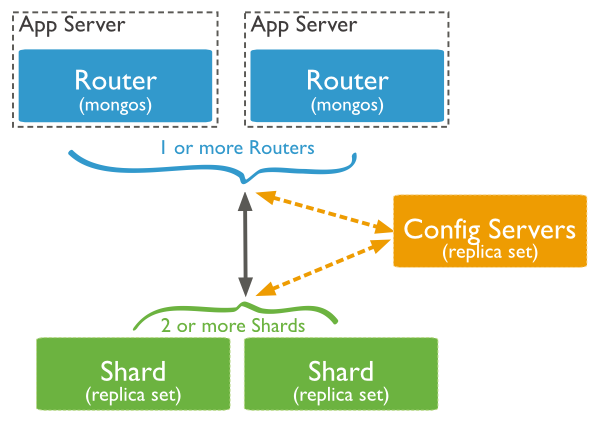
\includegraphics[scale=0.5]{images/sharded-cluster-production-architecture.png}
  \caption{Sharded MongoDB Architecture} \cite{www-mongoComponents}
\end{figure}

Figure 2 depicts a sharded MongoDB environment with two Mongos instances and two data Shards.  The replica sets shown for both Config Servers and Shards may have any number of replicas within the set.

\subsection{Config Servers}

Config Servers stored metadata for sharded MongoDB clusters.  This metadata includes information about the state and structure of the data and components of the sharded cluster. \cite{www-mongoConfig}

Config Servers also contain authentication information.  For example, information about the keyfiles used for internal authentication between the nodes (described in detail in the Security subsection that follow) is stored in the Config Servers. \cite{www-mongoConfig}

In production deployments, it is recommended for Config Servers to be deployed in 3 member replica sets. \cite{www-mongoComponents}  The rationale behind a 3 member set is discussed in more detail in the Replication subsection that follows.

In our deployment and benchmarking automation, the degree of replication in the Config Server Replica Set is controlled by the -c parameter.  For example, specifying 1 for -c will create a Replica Set with 1 Config Servers, specifying 1 for -c will create a Replica Set with 2 Config Server, and so on. 

\subsection{Mongos Routers}

Mongos is a query routing service used in sharded MongoDB configurations.  Queries from applications go through Mongos, which locates the data in the sharded cluster. The Mongos instances accomplish this by reading and caching data from the Config Servers. \cite{www-mongoMongos} 

For applications with high performance or availability requirements multiple Mongos instances may be ideal.  In a high volume application, spreading the routing load over multiple Mongos instances can benefit performance.  Additionally, multiple Mongos instances may increase availability in the case where a Mongos instance fails. \cite{www-mongoConfig}

In our deployment and benchmarking automation, the number of Mongos instances created is controlled by the -m parameter.  For example, specifying 1 for -m will create 1 Mongos instance, specifying 2 for -m will create 2 Mongos instances, and so on. 


\subsection{Shards}

Sharding, or distributing data across machines, is used by MongoDB to support large data sets and provide high throughput. \cite{www-sharding}.  Our deployment and benchmarking will test the performance of various numbers of shards, measuring the performance improvements associated with sharding in MongoDB.

Documents are distributed among the shards using a shard key.  A sharded collection must have one, and only one, shard key which must have a supporting index. \cite{www-sharding}  Since the shard key is critical to performance and efficiency, particular care must be given to shard key selection. \cite{www-shardkey} In our performance testing a key was chosen that would distribute data relatively evenly across the shards, but was not used in retrieving the data as the more costly retrieval of not using an index provided a better test case.

In our deployment and benchmarking automation, Sharding is controlled by the -s parameter.  For example, specifying 1 for -s will cause 1 shard to be created, specifying 2 will cause 2 shards to be created, and so on.

\subsection{Replication}

In databases, replication provides data redundancy leading to greater availability and fault tolerance.  Replication in MongoDB is achieved via Replica Sets. \cite{www-replication}  Replica Sets were implemented in our deployment for both Config Servers and Shards.

Two key benefits provided by replication are redundancy and fault tolerance.
\vspace{-\topsep}
\begin{itemize}
\item Redundancy - Each Replica in a Replica Set provides another copy of data.  Higher redundancy means more nodes can be lost without data being lost.
\item Fault Tolerance - Higher numbers of Replicas in a set increase fault tolerance, which leads to increased availability.  As a general rule, a set will be able to tolerate faults while the majority of its nodes are still available
\end{itemize}
\vspace{-\topsep}

\begin{figure}[ht]
\begin{center}
 \begin{tabular}{|c | c | c|} 
 \hline
Replica Members &  Majority Needed & Fault Tolerance \\ [0.5ex] 
 \hline\hline
    
2 &	1 &	0 \\
 \hline
3 &	2 &	1 \\ 
 \hline
4 &	3 &	1 \\ 
 \hline
5 &	3 &	2 \\ 
 \hline
6 &	4 &	2\\ 
 \hline
7 &	4 &	3\\ 
 \hline
8 &	5 &	3\\ [1ex] 
 \hline
\end{tabular}
\end{center}
  \caption{Fault Tolerance by Replica Set Size} \cite{www-mongoRepDep}
\end{figure}


As shown in Figure 3, odd numbers of members in a replica set are a better choice for fault tolerance. For example, both a 3 and 4 replace set can only tolerate one member failing while maintaining availability.  This is because a majority of the members must be available to maintain availability.  In a 3 replica set the majority is 2, so it can tolerate 1 member failing.  In a 4 replica set, the majority is 3, so it can still only tolerate 1 member failing.  Increases in fault tolerance only occur when the next odd numbered member of a replica set is added.  \cite{www-mongoRepDep}

For production systems, a standard deployment is a 3 Replica Set.  \cite{www-mongoRepDep}.  A 3 replica set provides 3 copies of the data for redundancy and fault tolerance if 1 member of the set were to fail.  In a situation where availability was of higher concern, a 5 replica set would provide 4 copies of the data for redundancy and fault tolerance if 2 members of the set were to fail.

In our automated deployment and benchmarking process, the degree of replication for Shards is controlled by the -r option. For example, specifying 1 for -r will create a replica set per shard with only 1 copy of data (essentially no replication, although technically we create a 1 member replica set), specifying 2 will cause a replica set of 2 to be created, and so on.

\subsection{Security}

There are two levels of security to consider in a sharded MongoDB deployment: internal and external authentication.

In our deployment the various MongoDB components (config servers, mongos instances, shards, and replicas) all reside on separate Virtual Machines.  These machines must be able to communicate with each other.  Two steps were necessary to enable this internal authentication.  First, the ports (27017, 27018, 27019, 28017) used by MongoDB needed to be opened for communication.  This was accomplished by adding appropriate security group rules to the clouds through Cloudmesh client.  Second, MongoDB requires the internal authentication to be done by either keyfiles or x.509 certificates.  \cite{www-mongoAuth}  In our deployment, authentication is done by keyfiles. CONSIDERING ADDING X.509 SECURITY OPTION

For external authentication, the three users were created.

\vspace{-\topsep}
\begin{itemize}
\item \emph{admin} - The user \emph{admin} is created with the role of \emph{userAdminAnyDatabase}.  This user performs administrative functions such as creating the other users.
\item \emph{cluster\_admin\_user} - The user \emph{cluster\_admin\_user} is created with the role \emph{clusterAdmin}. This user performs sharding functions such as sharding the collection and checking its data distribution.
\item \emph{user1} - This is a standard user with readWrite permissions.  This user performs the benchmarking tests and other functions not requiring administrative privileges.
\end{itemize}
\vspace{-\topsep}


\section{Deployment}

Will make major modifications

The automated process will fully deploy a sharded MongoDB environment with the number of Config Servers, Mongos Instances, Shards, and degree of Replication specified as input parameters.  It will also automatically created a sharded collection, run benchmarking tests agains it, and capture the output in CSV files as input for python visualization programs.

\subsection{Deployment Process}

The deployment consists of Ansible playbooks and Cloudmesh Client scripts and commands.  It is run on the user's local Ubuntu 16.04 instance and executes commands both locally and on virtual machines in the cloud over ssh.  A high level overview of the process is provided here.  An inventory and overview of the code used to automate the deployment process is provided in Appendix B.

The automated deployment is run by executing the top level script, mongo\_deploy.sh \cite{www-mongoDeploy} \cite{www-shardLocal} The script takes several parameters, described below.  The script will fully deploy the environment as specified.

THIS WILL DRASTICALLY CHANGE BUT LEAVING AS PLACEHOLDER TO MAKE SURE EVERYTHING IS INCLUDED AFTER CONVERSION TO ANSIBLE

\vspace{-\topsep}
\begin{itemize}
\item -d - the Deployment Cloud (\emph{chameleon} or \emph{kilo})
\item -c - a number, the size of Config Server Replica Set
\item -s - number of Shards
\item -r - a number, size of Shard Replica Set
\end{itemize}
\vspace{-\topsep}

After validating the input parameters the deployment is run as follows.

\textbf{Security}
\vspace{-\topsep}
\begin{enumerate}
\item Add and upload the user's public key (this functionality is currently disabled to prevent throwing an error as it is assumed the user has already done this).
\item Add security rules to the user's default security profile port opening ports 27107, 27018, 27019, and 28017 for communication.
\item Upload the security group profile.
\item Create a new random keyfile (described in more detail in the security section) for each deployment.
\end{enumerate}
\vspace{-\topsep}


\textbf{Config Servers}
\vspace{-\topsep}
\begin{enumerate}
\item Boot the appropriate number of Virtual Machines based on the -c parameter.
\item Check if there are available Floating IP Addresses in the pool.  If not, create a new one.
\item Assign a Floating IP to each Virtual Machine and record it in a file (the Floating IP is needed for communication between the servers and ssh from the client to the cloud).
\item Modify /etc/hosts to fix a warning message generated when running as sudo
\item Install MongoDB software on all servers.
\item Transfer the mongo.key file to the Virtual Machine using Secure Copy (scp)
\item Transfer a configuration file for the Config Server to the Virtual Machine using Secure Copy (scp)
\item Over ssh, stop the running mongod process on each server and start a new mongod processes using the configuration file sent in the previous step.
\item Over ssh, on one Config Server, run an initiate command including the IP addresses of the others to start the Replica Set.
\end{enumerate}
\vspace{-\topsep}


\textbf{Mongos Instances}
\vspace{-\topsep}
\begin{enumerate}
\item Boot the appropriate number of Virtual Machines based on the -m parameter.
\item Check if there are available Floating IP Addresses in the pool.  If not, create a new one.
\item Assign a Floating IP to each Virtual Machine and record it in a file (the Floating IP is needed for communication between the servers and ssh from the client to the cloud).
\item Modify /etc/hosts to fix a warning message generated when running as sudo
\item Install MongoDB software on all servers.
\item Transfer the mongo.key file to the Virtual Machine using Secure Copy (scp)
\item Transfer the configuration file for the mongos instance to each Virtual Machine using scp.  Prior to transferring, update the template configuration file to include the IP Address of the Configuration Server created earlier.
\item Over ssh, stop the running mongod process on each server and start a new mongos processes using the configuration file sent in the previous step.
\item Create several users (detailed in security section)
\end{enumerate}
\vspace{-\topsep}

\textbf{Shards}
\vspace{-\topsep}
\begin{enumerate}
\item For each -r Replica Set, boot the appropriate number of Virtual Machines based on the -s parameter.
\item Check if there are available Floating IP Addresses in the pool.  If not, create a new one.
\item Assign a Floating IP to each Virtual Machine and record it in a file (the Floating IP is needed for communication between the servers and ssh from the client to the cloud).
\item Modify /etc/hosts to fix a warning message generated when running as sudo
\item Install MongoDB software on all servers.
\item Transfer the mongo.key file to the Virtual Machine using Secure Copy (scp)
\item Transfer the configuration file for the Shard to each Virtual Machine using scp.  Prior to transferring, update the template configuration file to include the correct replica set name.
\item Over ssh, stop the running mongod process on each server and start a new mongod processes using the configuration file sent in the previous step.
\item Over ssh, on one shard in the replica set, run an initiate command including the IP addresses of the other shards in the set to start the Replica Set.
\item On a mongos instance, run a command to add the shard replica set.
\end{enumerate}
\vspace{-\topsep}



After deployment and benchmarking (described in detail in a later section) are complete, all Virtual Machines that have been created in the current deployment are deleted.

\subsection{Deployment Timing}

Will make major modifications

The configuration parameters and total deployment time is captured in a file for each deployment (benchmarking timings are later added to this file as well).  Total run time for a few interesting configurations are shown in Figure 4.  

Deployment A shows a simple deployment with only one of each component being created.  This deployment may only be suitable for a development or test environment.  Deployment A takes 517 seconds.

Deployment B shows a more complex deployment with production like replication factors for Config Servers and Shards and an additional Mongos instance.  This deployment may be suitable for a production environment as it has greater fault tolerance and redundancy.  Deployment B takes 2533 seconds.

Deployment C shows a deployment focused on high performance.  It has a high number of shards, 9, but no fault tolerance or redundancy.  The deployment may be suitable where performance needs are high and availability is less critical.  Deployment C takes 1968 seconds.

More detailed run times for these deployments are shown in Appendix B, along with benchmarking results.

\begin{figure}[ht]
%\begin{center}
\resizebox{\columnwidth}{!}{  
 \begin{tabular}{| c | c | c | c | c | c | c |} 
 \hline
 & Config Servers &  Mongos & Shards & Replicas & Time in \\
& -c &  -m & -s & -r & Seconds
\\ [0.5ex] 
 \hline
 \hline
 A & 1 & 1 & 1 & 1 & \emph{517} \\
 \hline
 B & 3 & 2 & 3 & 3 & \emph{2533} \\
 \hline
 C & 1 & 1 & 9 & 1 & \emph{1968} \\ [1ex] 
 \hline
\end{tabular}
}
%\end{center}
  \caption{Deployment Times on Chameleon Cloud in Seconds}
\end{figure}

The total number of virtual machines is highly correlated with deployment time as booting the machines and installing the software, tasks that occur for all nodes, take the most time.  he additional steps to configure Config Servers, Mongos Instances, Replicas, and Shards run in relatively similar times, so the specific type of component created has little impact on the deployment time.  For example, holding all other deployment variables at 1, a deployment with 5 Config Servers took 1258 seconds, one with 5 Mongos Instances took 1253 seconds, one with 5 Shards took 1292 seconds, and one with a 5 Shard Replica set took 1277 seconds.

Figure 5 shows this empirically, as it takes a very similar time to launch configurations with the same total number of nodes, but extremely different mixed of Config Servers, Mongos Instances, Replicas, and Shards.

The total number of nodes in a deployment can be calculated by the following equation involving the parameters to the deployment script.

c + m + ( s * r ) = total nodes

\begin{figure}[ht]
\begin{center}
 \begin{tabular}{| c | c | c | c | c | c |} 
 \hline
Config Servers &  Mongos & Shards & Replicas & Time in \\
-c &  -m & -s & -r & Seconds
\\ [0.5ex] 
 \hline
 \hline
\emph{5} & 1 & 1 & 1 & \emph{1258} \\
 \hline
 1 & \emph{5}  & 1 & 1 & \emph{1253} \\
 \hline
 1 & 1 & \emph{5} & 1 & \emph{1292} \\
 \hline
 1 & 1 & 1 & \emph{5}  & \emph{1277}  \\ [1ex] 
 \hline
\end{tabular}
\end{center}
  \caption{Deployment Times on Chameleon Cloud in Seconds}
\end{figure}

Note: Due to the floating IP issues in the Kilo environment, all deployment times shown are for Chameleon environment.  Professor von Laszewski is aware of these infrastructure issues and they cannot be resolved by the project team.  Fugang Wang is currently working on resolving them.


\section{Benchmarking}

After the sharded MongoDB instance has been fully deployed, a benchmarking process is run to assess performance of the configuration.  This process has also been fully automated.  It is automatically invoked after the deployment when running mongo\_deploy.sh.  An inventory of the code used to automate the benchmarking process is provided in Appendix B.


\subsection{Data Set}

Add Map/Reduce

The data set used in the benchmarking testing and analysis was Major League Baseball PITCHf/x data obtained by using the program Baseball on a Stick (BBOS).  \cite{www-bbos}  BBOS is a python program created by 
\emph{willkoky} on github which extracts data from mlb.com and loads it into a MySQL database.  While it would be possible to convert this program to populate the MongoDB database directly, collecting all of the data is a time consuming process. Therefore, the data was captured locally to the default MySQL database and then extracted to a CSV file.  This file contains 5,508,014 rows and 61 columns.  It is 1,588,996,075 bytes in size uncompressed.


\subsection{Methodology}

Will make major modications

The primary benchmarking goal of the project was to assess the impact of sharding on performance in MongoDB.  Since replication was also built into the deployment process, a secondary goal was to assess the impact of replica sets on performance.  The benchmarking tests are design to assess performance of the following situations.

MAY ADD MAP REDUCE TEST SCENARIO

https://docs.mongodb.com/manual/core/map-reduce/
https://docs.mongodb.com/manual/core/map-reduce-sharded-collections/

\vspace{-\topsep}
\begin{enumerate}
\item Impact of Sharding Configuration on Reads
\item Impact of Sharding Configuration on Writes
\item Impact of Replication Configuration on Reads
\item Impact of Replication Configuration on Writes
\end{enumerate}
\vspace{-\topsep}

To access the impact of different configurations on writes, we use MongoDB's mongoimport command.  Mongoimport is a command line tool capable of loading JSON, CSV, or TSV files. \cite{www-mongoimport} In this case, we load a CSV file to the pitches collections in the mlb database.

To assess the impact of different configurations on reads, we use MongoDB's find command.  We read the data previously loaded by the mongoimport command to the pitches collection.  The find command retrieves documents that meet a specified criteria.  In this case, we search for pitches with a speed over 100 mph, a relatively rare event in baseball.  To limit the information sent back over the network, we only return a count of these events.  3,632 is the count returned of 5,508,014 total documents.  The column we search on does not have an index, as the goal is to test the impact of sharding on a long running query.


For each test, timing results were captured in file benchmark\_datetime.csv.  This file included the configuration the MongoDB configuration the test was run under (cloud, config server replication factor, mongos instances, number of shards, and shard replication factor) along with the run times of the find and mongoimport commands.  After all tests were run, a shell script, combine\_benchmark.sh was run to combine all files into one file, benchmark\_combined.csv.

The graphical depictions of the test results show in the next section were created by running python programs to average the run times across the shard and replication configurations shown.  For consistency, config server replication and mongos instances were both kept at 1 for all benchmarking tests.  Additionally, replication was kept at 1 for sharding tests and sharding at 1 for replication tests.  This methodologies allows us to isolate the variable we are assessing.



A compressed version of file has been placed in an Amazon Web Services S3 directory.  The benchmarking script retrieves the file via wget, uncompresses it, and loads it to a collection named \emph{pitches} in MongoDB using mongoimport before running the find command.


\subsection{Benchmarking Process}

Before the benchmarking process can be run, a sharded collection must be created.  The script mongo\_collection.sh creates and shards a collection for the data set to be loaded to.  As with other steps in the process, this is automated and runs out of mongo\_deploy.sh.

\textbf{Create Sharded Collection}

\vspace{-\topsep}
\begin{enumerate}
\item Ssh to a mongos instance.  Authenticating as user1 via the mongo shell, create the pitches collection.
\item Ssh to a mongos instance.  Authenticating as cluster\_admin\_user via the mongo shell, run a command to enable sharding in the mlb database the pitches table is located in.
\item Ssh to a mongos instance.  Authenticating as cluster\_admin\_user via the mongo shell, run a command to shard the collection.  
\end{enumerate}
\vspace{-\topsep}

The shard key is set to pitchID.  PitchID is a unique key to each pitch document.  Selecting pitchID as the shard key should cause the data to be reasonably evenly distributed amound the shards.  Data distribution will be analyzed in a subsequent section.

Once the sharded collection has been created, benchmarking test can be run.  The script mongo\_benchmark.sh runs the benchmarking process.  It adds the benchmarking times for both find and mongoimport to the file created during the deployment containing the configuration parameters and deployment time.

\textbf{Benchmarking}


\vspace{-\topsep}
\begin{enumerate}
\item Ssh to a mongos instance.  Using wget retrieve the pitches file from a Amazon Web Services (AWS) Simple Storage Service (S3) folder and uncompress the file.
\item Connect to a mongo shell on the mongos instance and run a mongoimport of the file to the sharded collection, capturing the run time.
\item Connect to a mongo shell on the mongos instance and run a find command against the sharded collection, capturing the run time. 
\end{enumerate}
\vspace{-\topsep}


\subsection{Data Distribution}

To explore how data was allocated among the shards, the getShardDistribution() command, which reports on how data and documents are distributed among shards \cite{www-shardDist}, is run as part of the automated process after the data is populated in the collection by mongoimport.  Figure 6 show the results of tests with 1 to 5 shards.  The results clearly show the data is well distributed, although interestingly, in all cases there is some skew toward the final shard having the most data.


\begin{figure}[ht]
\begin{center}
 \begin{tabular}{| c | c | c | c | c | c |} 
 \hline
  &  1    &  2    &  3    &   4   & 5 \\ [0.5ex]
\hline
  \hline
1 & 100   &       &       &       &   \\
\hline
2 & 45.83 & 54.16 &       &       &   \\
\hline
3 & 31.17 & 31.05 & 37.76 &       &   \\
\hline
4 & 23.72 & 23.98 & 24.14 & 28.14 &   \\
\hline
5 & 19.27 & 18.88 & 18.86 & 18.89 & 24.08   \\
\hline
\end{tabular}
\end{center}
  \caption{Data Distribution among Shards}
\end{figure}





\subsection{Benchmarking Analysis}

\subsubsection{Impact of Sharding on Reads}

\begin{figure}[!ht]
  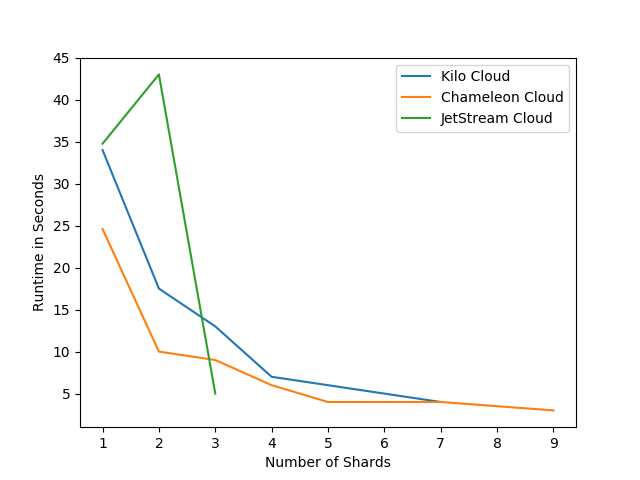
\includegraphics[scale=0.45]{images/shard_find.png}
  \caption{Find Command - Sharding Test}
\end{figure}

Will make major modications

Figure 7 depicts the impact on performance of various numbers of shards on a find command in both Chameleon and Kilo Clouds.  The sharp decline in run time as the number of shards is increased shows the positive effect of sharding on performance.  For example, while the run time for 1 shard in both Chameleon and Kilo is over 120 seconds, the time drops to around 15 seconds for 6 shards.  This is a significant gain in performance.  

For small numbers of shards, performance gains are almost exact proportion to the number of shards.  2 shards yields 1/3 the run time of 1 shard.  3 shards yields 1/2 the run time of 1 shard.  From 3 to 6 chards, we still see still see significant improvement, but incrementally less than for the first 3 shards.  After 6 shards, we see only slight performance gains.

From the closeness of the Chameleon and Kilo lines we can see that performance in the two clouds is very similar for this find test.  This is an interesting observation as for both deployment and mongoimport, performance was much better on Chameleon Cloud than Kilo.  One difference from the mongoimport test is that much less data is being sent over the network.  Network speeds could be a factor in this discrepency.

Figure 7 can be recreated by running the program benchmark\_shards\_find.py passing the file benchmark\_combined.csv as a parameter.  It plots the average run time for each configuration as shown using matplotlib.



\subsubsection{Impact of Sharding on Writes}

Will make major modications

\begin{figure}[!ht]
  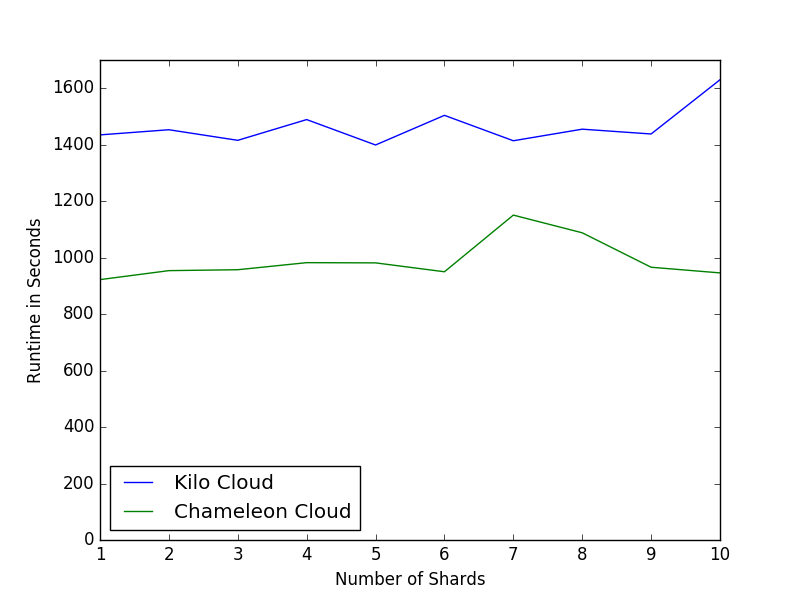
\includegraphics[scale=0.45]{images/shard_import.png}
  \caption{Mongoimport Command - Sharding Test}
\end{figure}


Figure 8 depicts the impact on performance of various numbers of shards on a mongoimport command in both Chameleon and Kilo Clouds.  For both clouds run time of the mongoimport command in our tests does not appear to be  impacted by the number of shards.  Since the same amount of data is written with more computing resources available when there are more shards, we might expect to see a performance gain.  However, there are possible explanations for performance not improving.  First, the mongoimport command may not write data in parallel.  This is not indicated in the documentation, but it seems likely that it reads the file serially.  Second, resources on the server the data is written to may not be the bottleneck in the write process.  Other resources like the network time are likely to be the bottleneck.  Since we are always going over the network from the mongos instance to a data shard, regardless of the number of shards, a bottleneck in the network would impact all shard configurations equally.

While sharding did not benefit a single threaded mongoimport command, it is likely it would benefit heavy write operations, particularly coming through multiple mongos instances.  In a non-sharded environment, this would lead to a heavy load on the single data shard.  In a sharded environment, the load on each shard would drop as the number of shards increased.

While performance on Chameleon and Kilo was very similar for the find command, performance of the mongoimport command was significantly better on Chameleon than on Kilo.  We see approximately 50\% better performance on Chameleon Cloud than on Kilo.  Although not formally plotted due to environmental issue in Kilo Cloud, similar results were observed for deployment times.  Overall, Chameleon Cloud is a faster environment that FutureSystems Kilo Cloud.

Figure 9 can be recreated by running the program benchmark\_shards\_import.py passing the file benchmark\_combined.csv as a parameter.  It plots the average run time for each configuration as shown using matplotlib.




\subsubsection{Impact of Replication on Reads}

Will make major modications

\begin{figure}[!ht]
  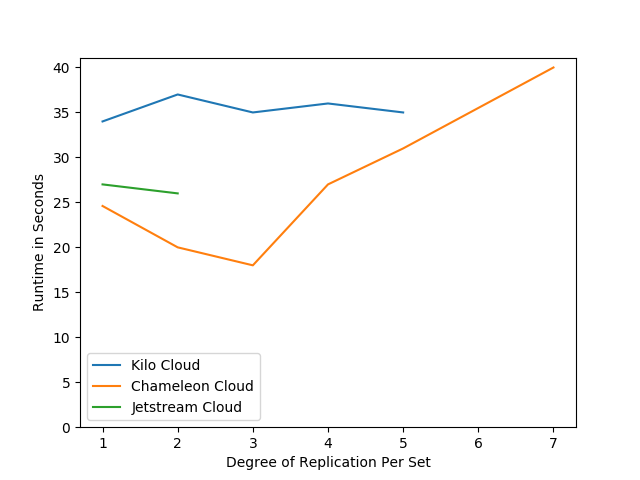
\includegraphics[scale=0.45]{images/replica_find.png}
  \caption{Find Command - Replication Test}
\end{figure}


Figure 9 depicts the impact on performance of various numbers of replicas on a find command in both Chameleon and Kilo Clouds.  (Note: Due to environmental issues with floating IPs in the India/Kilo environment, tests were only able to be run from 1, 2, and 3 replica configurations on Kilo cloud.  This is an infrastructure problem beyond the control of the project team that Professor von Laszewski is aware of.)  While it is clear that replication does not have the same performance impact on the find command that sharding does, it appears that there may be a slight performance penalty to high degrees of replication.  Replica sets up to 3 did not show this penalty, but 4 and 7 replica sets both had increased run times.  Without a larger sample size it cannot be determined if this is a real effect or random variation.  We would not expect replication to have a significant performance degradation on the the find command since it only needs to read one copy of the data, but the increased communication necessary in a replica set may cause a small performance penalty in some cases.

Similarly to our sharding mongoimport test, performance on Chameleon was better than on Kilo for all test runs in the find replication test.  The difference was similar to the 50\% improvement noted earlier.

Figure 9 can be recreated by running the program benchmark\_replicas\_find.py passing the file benchmark\_combined.csv as a parameter.  It plots the average run time for each configuration as shown using matplotlib.



\subsubsection{Impact of Replication on Writes}

Will make major modications

\begin{figure}[!ht]
  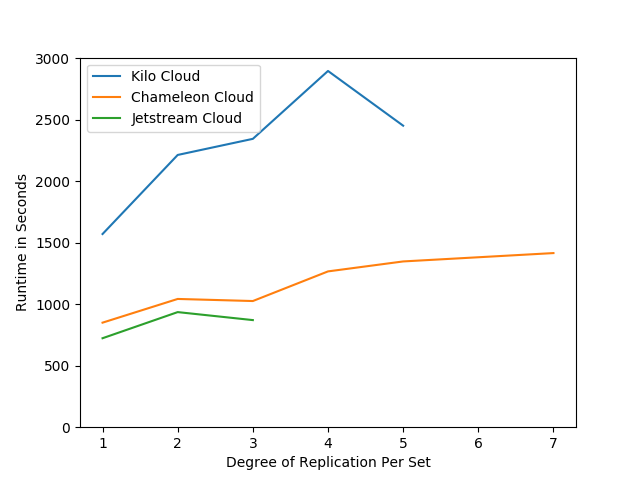
\includegraphics[scale=0.45]{images/replica_import.png}
  \caption{Mongoimport Command - Replication Test}
\end{figure}


Figure 10 depicts the impact on performance of various numbers of replicas on a mongoimport command in both Chameleon and Kilo Clouds.  (Note: Due to environmental issues with floating IPs in the India/Kilo environment, tests were only able to be run from 1, 2, and 3 replica configurations on Kilo cloud.  This is an infrastructure problem beyond the control of the project team that Professor von Laszewski is aware of.)  The test results show negative impact on the mongoimport command for increase levels of replication.  On Chameleon, a replication factor of 2 leads to approximately a 20\% performance penalty and a replication factor of 7 leads to 50\% worse performance.  Given that an extra copy of data is written with each increase in the replication factor, this performance hit is expected.  

Similarly to our sharding mongoimport and find replication tests, performance on Chameleon was better than on Kilo for all test runs in the mongoimport replication test, again by a similar percentage.

Figure 10 can be recreated by running the program benchmark\_shards\_import.py passing the file benchmark\_combined.csv as a parameter.  It plots the average run time for each configuration as shown using matplotlib.



\section{Summary}

Will make major modications

We have created, tested, and demonstrated a fully automated program to configure and deploy a sharded MongoDB cluster to three cloud environments.  The cluster can be deployed with a selected number of Config Server Replicas, Mongos Routers, Shards, and Shard Replicas.  An automated benchmarking process to show the impact of well distributed data across shards of a large data set has been created and run for various configurations to assess the impact of Sharding and Replication on performance.  A key finding of these tests is that read performance, typically a high priority for noSQL data stores, increases significantly as shards are added.  Testing also showed a predictable performance penalty is associated with replication.




\section*{Acknowledgements}

Funding information should be listed in this section. Please evaluate
if you like to list your employer that may have funded your activities
here.  If you receive grants or project numbers, as shown in the
example.  This work was in part supported by National Science
Foundation (NSF) (1234567, 891012345) (These numbers are invented)

The acknowledgments may also contain any information that is not
related to funding:

The authors thank H. Haase, C. Wiede, and J. Gabler for technical
support.


% Bibliography

\bibliography{references}
 
\section*{Author Biographies}
\begingroup
\setlength\intextsep{0pt}
\begin{minipage}[t][3.2cm][t]{1.0\columnwidth} % Adjust height [3.2cm] as required for separation of bio photos.
  \begin{wrapfigure}{L}{0.25\columnwidth}
    
\includegraphics[width=0.25\columnwidth]{images/john_smith.eps}
  \end{wrapfigure}
  \noindent
{\bfseries Mark McCombe} received his B.S. (Business Administration/Finance) and M.S. (Computer Information Systems) from Boston University.  He is currently studying Data Science at Indiana University Bloomington.

\end{minipage}
\endgroup

\newpage

\appendix

\section{Work Breakdown}

The work on this project was distributed as follows between the
authors:

\begin{description}

\item[Mark McCobme.] Completed all work.

\end{description}


\end{document}
